\chapter{Application description}\label{chapter:appdescription}


\section{Requirements}
The application can be used in different area of application. The main requirement is to have a smartphone with a camera and a QR code reader. The application is available for Android and iOS. The application is available for free on the Google Play Store and the Apple App Store. The application is available in English and Romnian. The users will be able to import any model in the application using the QR code.

\section{Description}
\pagebreak
\section{Diagrams}
\subsection{Use cases}
Each user that has a smartphone capable to run the AR moduls should be able to use the app. If the user has models already imported he/she can use the app without any connection to the internet. If the user wants to import a new model he/she will need to have an internet connection. The user will be able to import a model using the QR code. The user will be able to see the model in AR mode. The user will be able to see the guide of the model. The user will be able to see the list of all the models that he/she has imported. The user will be able to delete a model from the list of models. The user will be able to see the list of all the models that he/she has imported. The user will be able to delete a model from the list of models.
\begin{figure}[h!]
    \begin{center}
        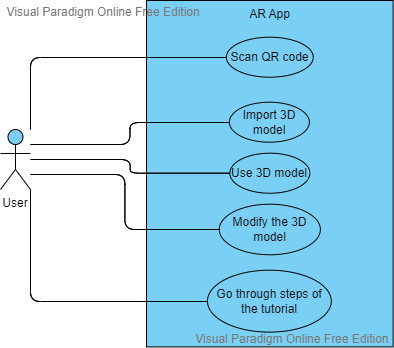
\includegraphics{img/InitialUseCase.png}
        \caption{Initial use case}
        \label{fig:InitialUseCase}
    \end{center}
\end{figure}
\pagebreak

\subsection{Sequence diagram}
TEXT TO BE ADDED
\begin{figure}[h!]
    \begin{center}
        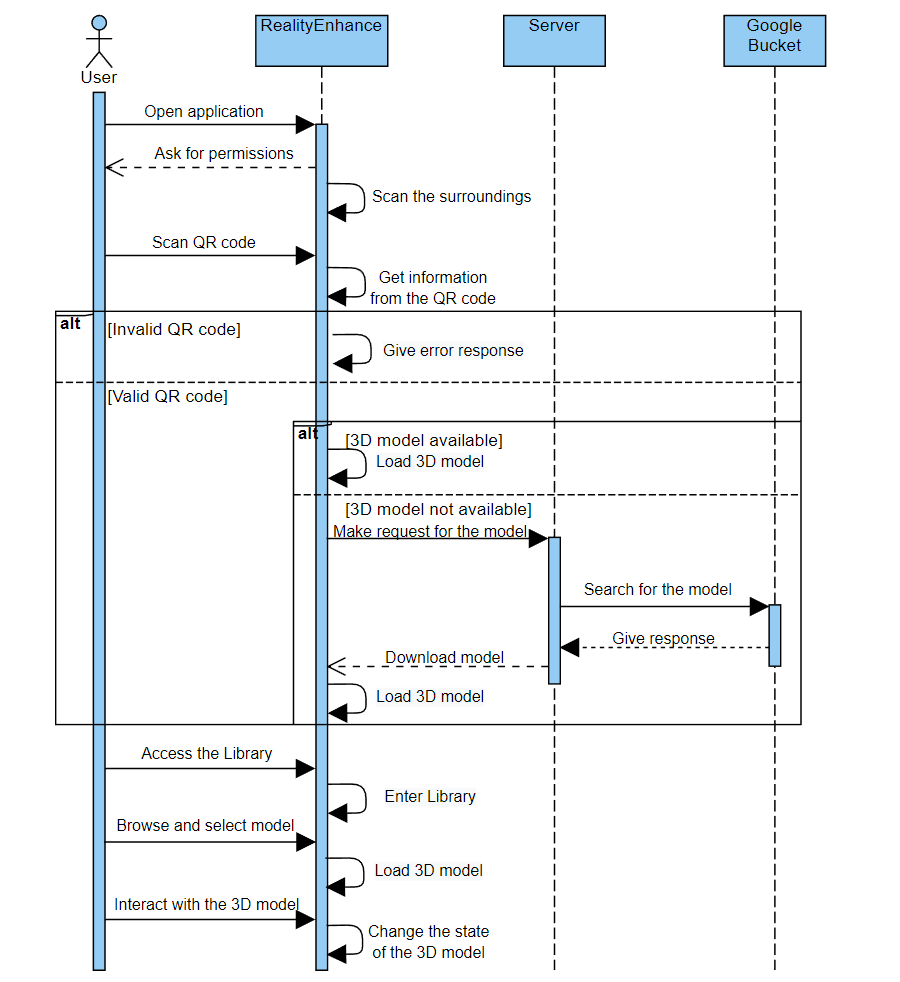
\includegraphics{img/SequenceDiagram.png}
        \caption{Sequence diagram}
        \label{fig:SequenceDiagram}
    \end{center}
\end{figure}

\section{Features}
\subsection{Import model}
\subsection{See model in AR}
\subsection{See guide}
\subsection{See list of models}
\subsection{Delete model}
\subsection{Load model from library}
\subsection{Create a scene}


\section{Architecture}
The application will be developed using the Android Studio IDE. The application will be developed using the Java programming language. The application will use the Google ARCore framework. The application will use the Firebase cloud database to store the models. The application will use the QR code reader to import the models. The application will use the Google Vision API to recognize the QR code.
\begin{figure}
    \begin{center}
        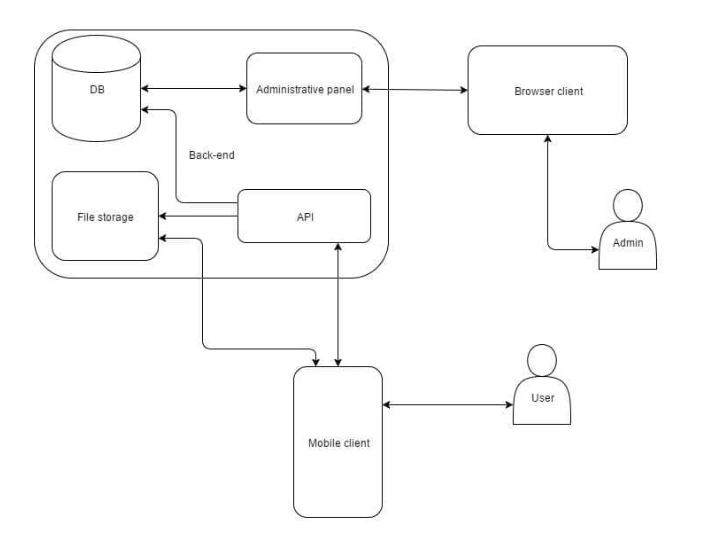
\includegraphics{img/architecture.png}
        \caption{Architecture}
        \label{fig:architecture}
    \end{center}
\end{figure}

\begin{itemize}
    \item \textbf{Android Version 7.0+} - to use the application on the phone
    \item \textbf{Android Studio} - IDE for Android development
    \item \textbf{Firebase} - Cloud DataBase for where the models will be retrieved
    \item \textbf{Java} - Programming language
    \item \textbf{Google ARCore} - AR framework
\end{itemize}

\section{Implementation}

\section{Testing}

\section{Deployment}

\section{Maintenance}

